\documentclass[12pt,letterpaper]{article}

\usepackage[margin=1in]{geometry}
\usepackage{setspace}
\usepackage{amsmath,amssymb}
\usepackage{graphicx}
\usepackage{booktabs}
\usepackage[font={normalsize,stretch=2},labelfont=bf]{caption}
\usepackage[hidelinks]{hyperref}

\doublespacing
\setlength{\parindent}{0.5in}
\setlength{\parskip}{0pt}

% Guidelines: at most 10 double-spaced pages, including tables and figures.
% Introduction: at most 2 pages. Conclusion: at most 1 page.
% Keep text, captions, tables, and references at least 12 pt and double-spaced.
% Use processed results, rather than raw data, in the report.
% Number and caption every figure/table; refer to each in your own text.
% Define variables, state units, and use appropriate significant digits.

\begin{document}

\hypersetup{pageanchor=false}
\begin{titlepage}
    \centering
    \vspace*{1.5cm}
    {\Large\bfseries Lab 1 -- Ideal Gas Law\par}
    \vspace{0.5cm}
    {\large CHE 260 -- Thermodynamics and Heat Transfer\par}
    \vspace{1.5cm}

    \textbf{Group Members}\par
    % Add or remove rows to match the group size; fill in every name and ID.
    \begin{tabular}{@{}p{0.45\textwidth}p{0.35\textwidth}@{}}
        \textbf{Chance Hattrick} & \textbf{Student ID} \\
        \textbf{Ammar Hasham} & \textbf{Student ID} \\
        \textbf{Muhammad Hasnain Heryani} & \textbf{1011884695} \\
    \end{tabular}

    \vspace{1cm}
    \textbf{PRA Section: PRA0103}\par
    \textbf{Experiment Date: September 30th, 2026}\par
    \textbf{Submission Date: Oct 8th, 2026}\par
    \vfill
\end{titlepage}
\hypersetup{pageanchor=true}

\section{Introduction}
% Introduce the subject, objectives, main observations, and relevant theory.
% Maximum 2 pages.

\section{Results and Discussion}

\subsection{Part 1: Path Independence and Tank Volume Ratio}

Part 1 of the lab discusses the comparison between the movement of air between two identical volume tanks, 
one with a gauge pressure of 40 PSI to another with a gauge pressure of 0-PSI.\@The main point of comparison 
is the differences in a slow equalization of pressure versus a rapid equalization of pressure.\@


\subsubsection{Processed Results: Rapid and Slow Expansion}
Figures~\ref{fig:part1a-pressure}--\ref{fig:part1b-flow} show the measured pressure, temperature, and mass-flow histories for the rapid and slow expansions.

\begin{figure}[!htbp]
    \centering
    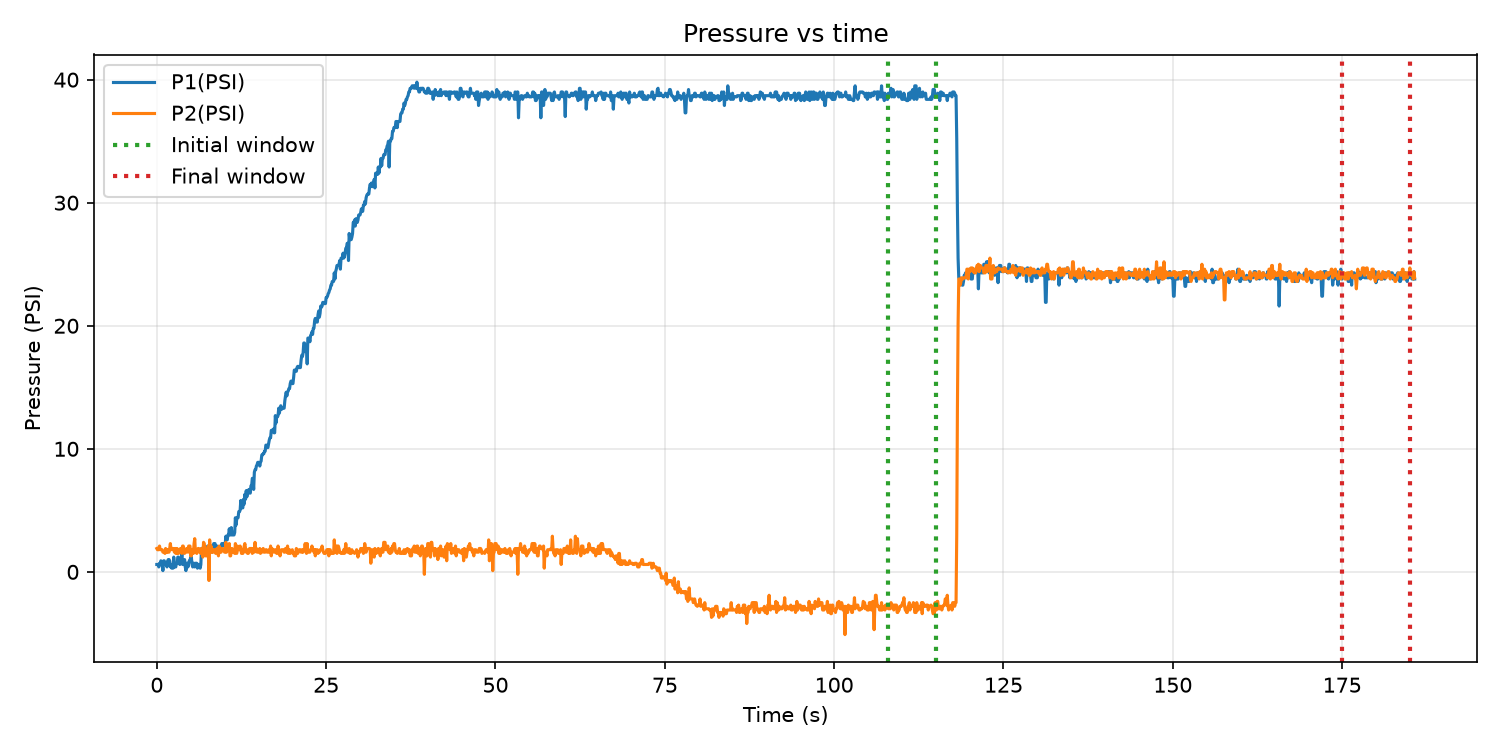
\includegraphics[width=0.82\linewidth,height=0.27\textheight,keepaspectratio]{lab-part1a_plots/pressure.png}
    \caption{Tank pressures during the Part 1a rapid expansion.}
    \label{fig:part1a-pressure}
\end{figure}

\begin{figure}[!htbp]
    \centering
    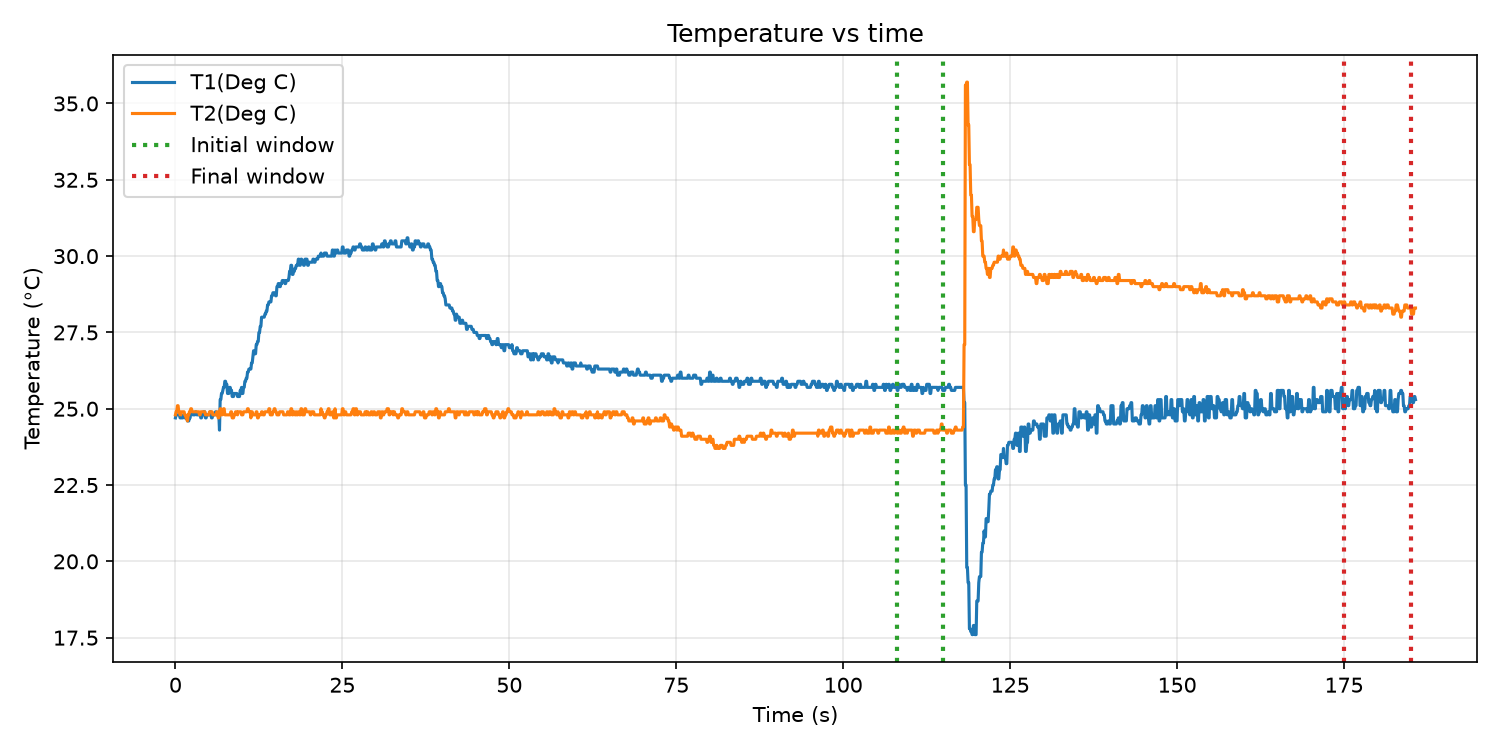
\includegraphics[width=0.82\linewidth,height=0.27\textheight,keepaspectratio]{lab-part1a_plots/temperature.png}
    \caption{Tank temperatures during the Part 1a rapid expansion.}
    \label{fig:part1a-temperature}
\end{figure}

\begin{figure}[!htbp]
    \centering
    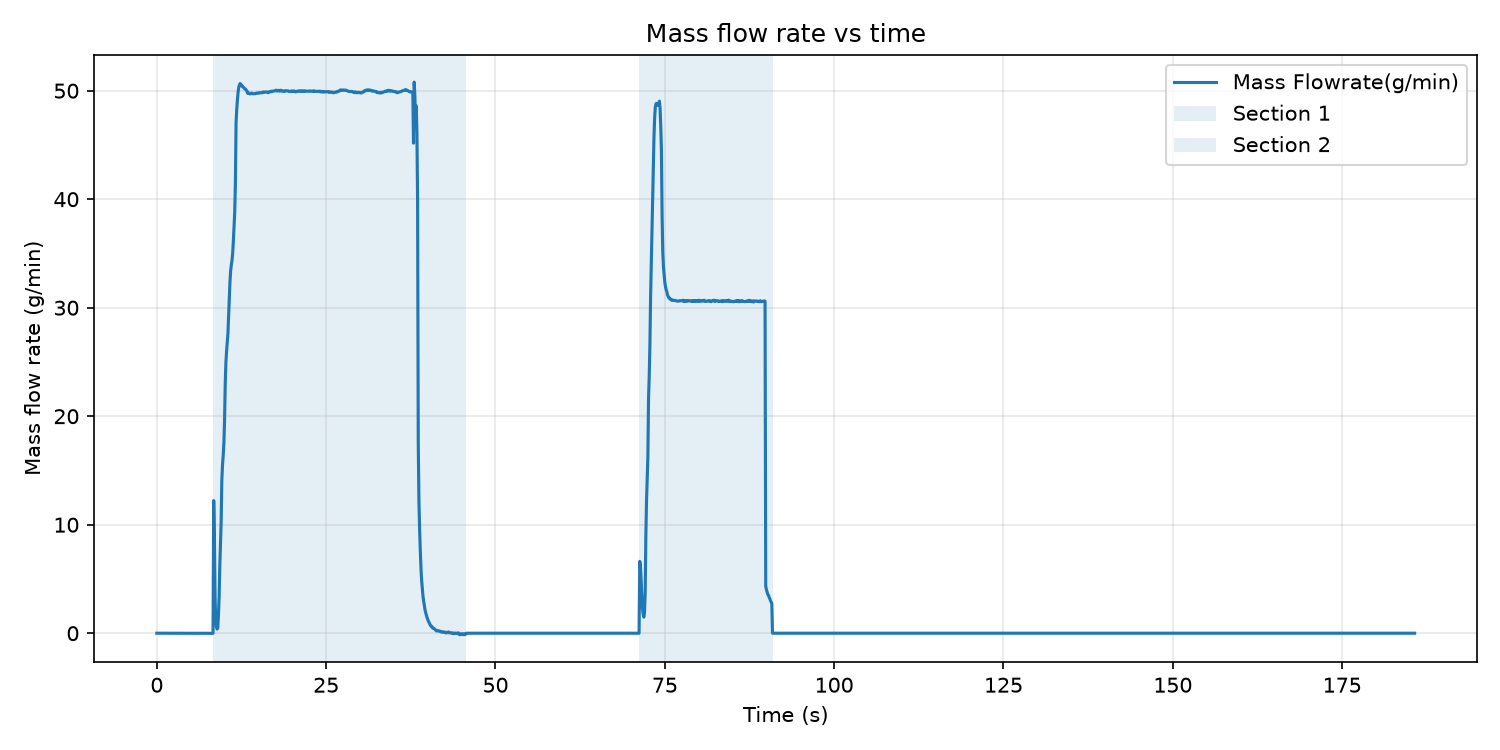
\includegraphics[width=0.82\linewidth,height=0.27\textheight,keepaspectratio]{lab-part1a_plots/mass_flow_rate.png}
    \caption{Mass flow rate during the Part 1a rapid expansion.}
    \label{fig:part1a-flow}
\end{figure}

\begin{figure}[!htbp]
    \centering
    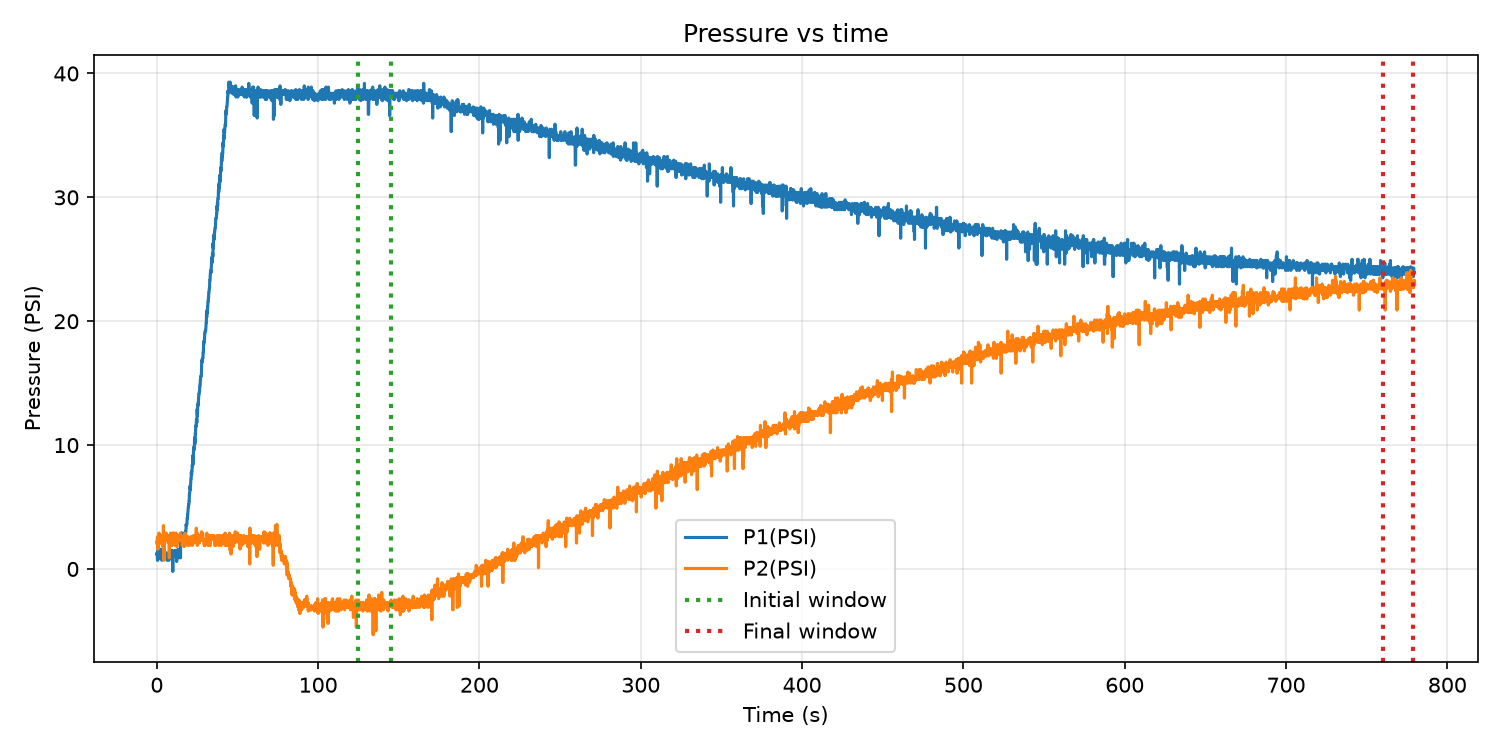
\includegraphics[width=0.82\linewidth,height=0.27\textheight,keepaspectratio]{lab-part1b_plots/pressure.png}
    \caption{Tank pressures during the Part 1b slow expansion.}
    \label{fig:part1b-pressure}
\end{figure}

\begin{figure}[!htbp]
    \centering
    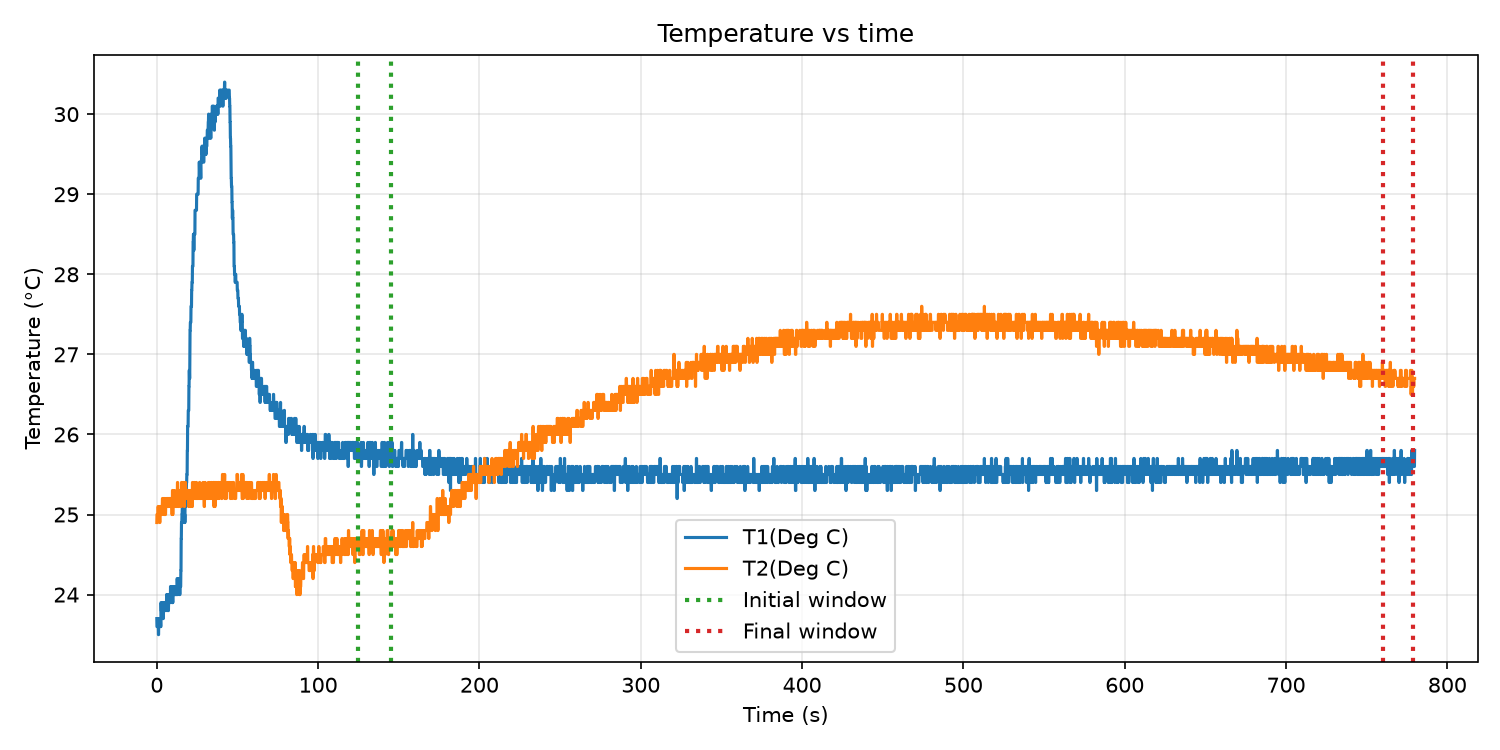
\includegraphics[width=0.82\linewidth,height=0.27\textheight,keepaspectratio]{lab-part1b_plots/temperature.png}
    \caption{Tank temperatures during the Part 1b slow expansion.}
    \label{fig:part1b-temperature}
\end{figure}

\begin{figure}[!htbp]
    \centering
    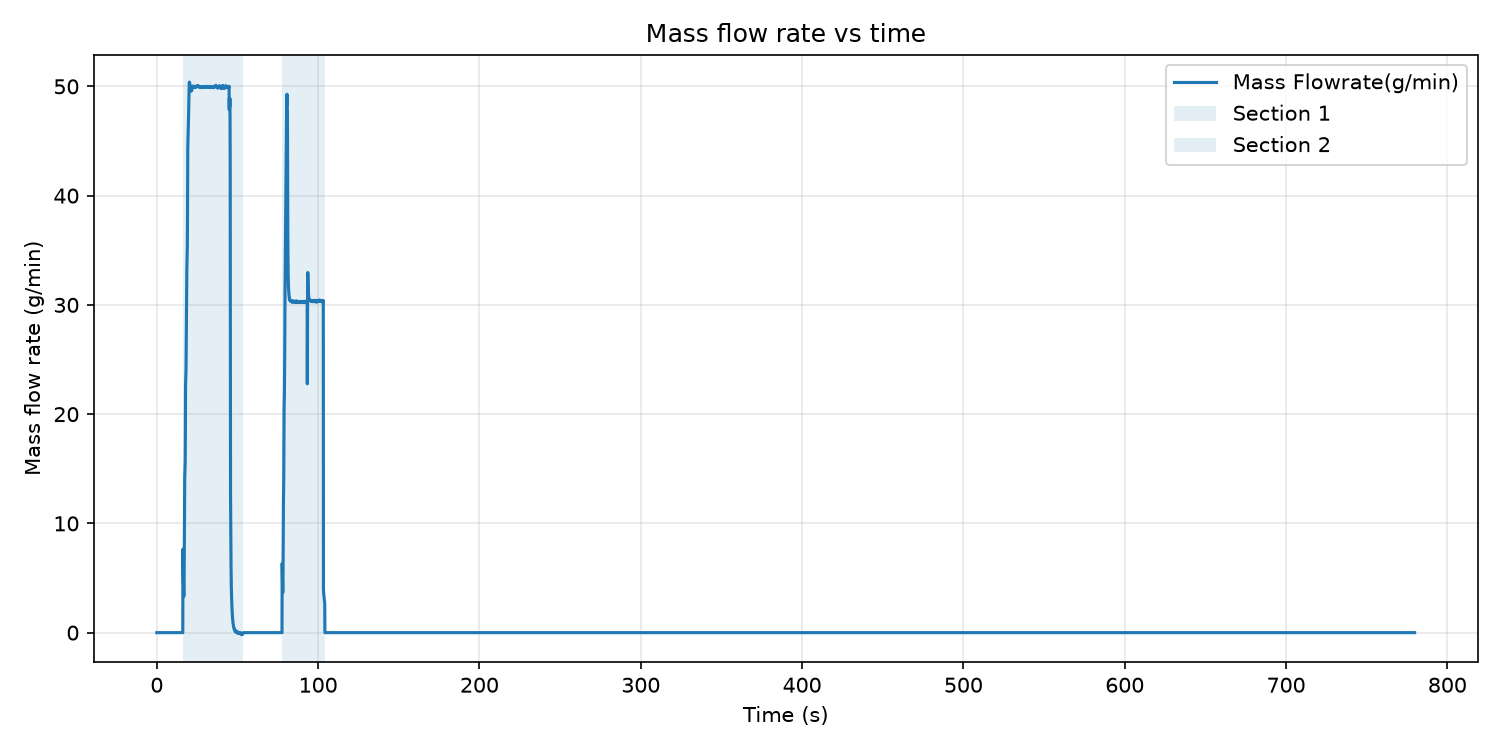
\includegraphics[width=0.82\linewidth,height=0.27\textheight,keepaspectratio]{lab-part1b_plots/mass_flow_rate.png}
    \caption{Mass flow rate during the Part 1b slow expansion.}
    \label{fig:part1b-flow}
\end{figure}

\clearpage
% Identify initial and final pressure/temperature states for both tanks.

\subsubsection{Tank Volume Ratio}
% Part 1, Question 1: ideal gas law and conservation of mass.
% Space for derivation, representative calculation, and results.

\subsubsection{Heat Transfer and Net Heat Transfer}
% Part 1, Question 2: explain heat transfer with surroundings for both cases.
% Discuss net heat transfer; the handout does not require calculations here.

\subsubsection{Path Independence of State Properties}
% Part 1, Question 3: compare the two paths and their final states.
% Include and reference a figure supporting the explanation.

\subsection{Part 2: Initial Mass and Volume of the Left Tank}

\subsubsection{Processed Pressure, Temperature, and Mass Flow Results}
% Insert numbered, captioned graphs/tables for Part 2.
% Identify the integration interval and the states used in calculations.

\subsubsection{Initial Mass and Tank Volume}
% Part 2, Question 1: space for mass-flow integration and calculations.
% Distinguish initial mass, added mass, and final mass in your analysis.
% Include a representative calculation and identify all variables/units.

\subsubsection{Sources of Error and Limitations}
% Part 2, Question 2: discuss sources of error and their effects on results.
% Address relevant assumptions and limitations for both lab parts.

\subsubsection{Effect of Air Compressibility}
% Part 2, Question 3: discuss the effect on the calculated results.

\section{Conclusion}
% Summarize the major experimental outcomes/findings. Maximum 1 page.

\section*{References}
\phantomsection
% Replace this heading with thebibliography when adding references:
% \begin{thebibliography}{99}
% \bibitem{key} ...
% \end{thebibliography}
% Cite using \cite{key}; number sources in order of first appearance.
% Journal: Author(s), Journal Title. Volume (Year) Page number.
% Book: Author(s), Book Title. Publisher, City, Year, Page(s).
% Website: website address.
% Course notes: Author or Course Name. Title of Document. Year Accessed.
% Acknowledge AI-assisted outlining in the references using:
% Tool Name, URL, Date used, Description how it was used, Prompt(s) used.
% Record the actual tool/date and the prompt used for this template.

% If using generative AI as a source, the guidelines require a screenshot
% of its output in an appropriately titled appendix. Enable if applicable:
% \appendix
% \section{AI Output Documentation}
% Insert the required screenshot here and check the total page limit.

\end{document}
